\documentclass[tikz,border=10pt]{standalone}
\begin{document}
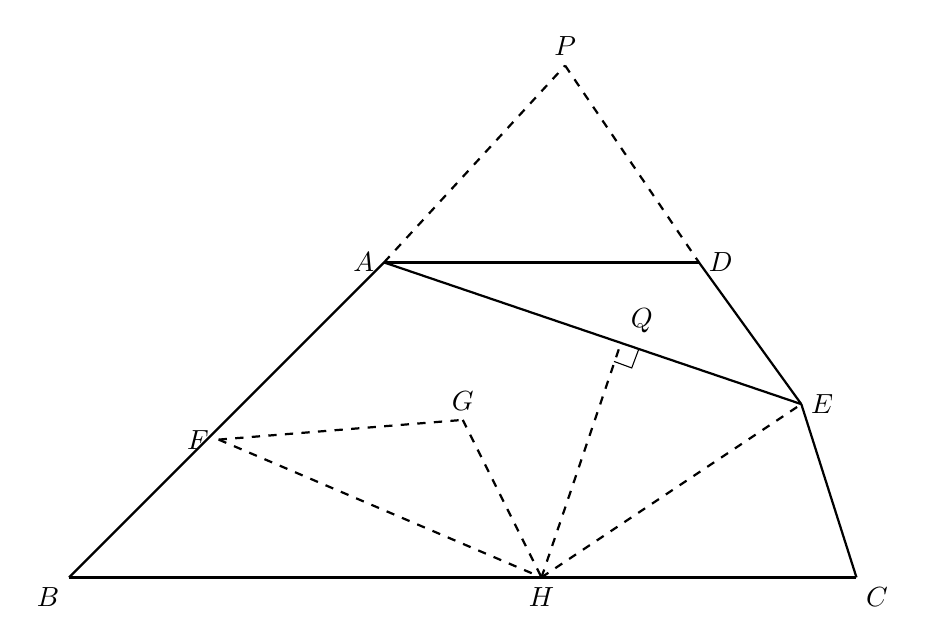
\begin{tikzpicture}
  \coordinate (B) at (0,0);
  \coordinate (C) at (10,0);
  \coordinate (H) at (6,0);
  \coordinate (A) at (4,4);
  \coordinate (D) at (8,4);
  \coordinate (P) at (6.3,6.5);
  \coordinate (F) at (1.9,1.75);
  \coordinate (G) at (5,2);
  \coordinate (E) at (9.3,2.2);
  \coordinate (Q) at (7.01,2.98);

  % solid edges
  \draw[thick] (B) -- (A);
  \draw[thick] (A) -- (D);
  \draw[thick] (A) -- (E);
  \draw[thick] (D) -- (E);
  \draw[thick] (E) -- (C);
  \draw[thick] (B) -- (C);

  % dashed edges
  \draw[dashed,thick] (A) -- (P);
  \draw[dashed,thick] (P) -- (D);
  \draw[dashed,thick] (F) -- (G);
  \draw[dashed,thick] (G) -- (H);
  \draw[dashed,thick] (F) -- (H);
  \draw[dashed,thick] (H) -- (Q);
  \draw[dashed,thick] (H) -- (E);

  % right angle mark at Q
  \draw (7.236,2.90) -- (7.146,2.66) -- (6.92,2.743);

  % labels
  \node[below left] at (B) {$B$};
  \node[below right] at (C) {$C$};
  \node[below] at (H) {$H$};
  \node[left] at (A) {$A$};
  \node[right] at (D) {$D$};
  \node[above] at (P) {$P$};
  \node[left] at (F) {$F$};
  \node[above] at (G) {$G$};
  \node[right] at (E) {$E$};
  \node[above right] at (Q) {$Q$};
\end{tikzpicture}
\end{document}
